\chapter{La reproduction sexuée des plantes à fleurs}\label{ch:b2:angiosperm-reproduction}

Un verger de pommiers est blanc de \omterm{def:b2:angiosperm-reproduction:flower}{fleurs} en mai et bourdonnant
d'abeilles~; en octobre, les mêmes arbres ploient sous les \omterm{def:b2:angiosperm-reproduction:seed}{fruits}, chaque
pomme contenant dix pépins, chaque pépin étant un embryon d'arbre
enveloppé dans une réserve de nourriture. Toute cette transformation
--- la \omterm{def:b2:angiosperm-reproduction:flower}{fleur}, le \omterm{def:b2:plant-life-cycles:heterospory}{pollen} transporté par un insecte, le tube qui traverse
le style, la \omterm{prop:b2:angiosperm-reproduction:double}{double fécondation} qui produit à la fois un embryon et sa
réserve nutritive, l'\omterm{def:b2:angiosperm-reproduction:flower}{ovaire} qui gonfle en un \omterm{def:b2:angiosperm-reproduction:seed}{fruit} fait pour être mangé
--- est l'invention qui a fait des plantes à \omterm{def:b2:angiosperm-reproduction:flower}{fleurs}, en cent millions
d'années, les plantes dominantes de la terre ferme. Ce chapitre la suit
de la \omterm{def:b2:angiosperm-reproduction:flower}{fleur} à la \omterm{def:b2:angiosperm-reproduction:seed}{graine} dispersée.

\section{La fleur}

\begin{definition}[Les pièces florales]\label{def:b2:angiosperm-reproduction:flower}
\index{fleur}\index{etamine@étamine}\index{carpelle}\index{ovaire}\index{stigmate}
Une \emph{fleur} est un rameau court dont les feuilles sont
transformées en quatre verticilles. À l'extérieur, les \emph{sépales}
(ensemble, le calice) protègent le bouton~; puis les \emph{pétales} (la
corolle), qui attirent~; puis les \emph{étamines}, formées chacune d'un
filet portant une \emph{anthère} à quatre sacs polliniques~; et au
centre un ou plusieurs \emph{carpelles}, chacun replié et soudé en un
\emph{pistil} pourvu d'un \emph{stigmate} réceptif, d'un \emph{style} et
d'un \emph{ovaire} qui renferme les \emph{\omterm{def:b2:plant-life-cycles:heterospory}{ovules}}. Une fleur portant à
la fois étamines et carpelles est \emph{hermaphrodite} (la plupart des
espèces)~; les plantes \emph{monoïques} portent des fleurs mâles et des
fleurs femelles séparées sur un même individu (maïs, chêne, noisetier),
les espèces \emph{dioïques} sur des individus distincts (houx, saule,
palmier dattier). Tout l'intérêt du carpelle clos --- le caractère qui
donne leur nom aux angiospermes --- est que les \omterm{def:b2:plant-life-cycles:heterospory}{ovules} sont enfermés~:
le \omterm{def:b2:plant-life-cycles:heterospory}{pollen} ne les atteint jamais directement, mais doit croître jusqu'à
eux à travers les tissus de la plante, ce qui permet à celle-ci de
choisir.
\end{definition}

\begin{omfigure}
\begin{tikzpicture}[every node/.style={font=\scriptsize}]
  % receptacle and pedicel
  \draw[thick] (0,-2.6) -- (0,-1.6);
  \draw[thick, fill=omExo!20] (-0.9,-1.6) .. controls (-1.0,-1.0) and (1.0,-1.0) .. (0.9,-1.6) -- cycle;
  % sepals
  \foreach \s in {-1,1} \draw[thick, fill=omExo!45] (0.6*\s,-1.4) .. controls (2.0*\s,-1.2) and (2.6*\s,-0.2) .. (2.8*\s,0.6) .. controls (2.0*\s,0.2) and (1.2*\s,-0.6) .. (0.6*\s,-1.4);
  % petals
  \foreach \s in {-1,1} \draw[thick, fill=omThm!15] (0.5*\s,-1.2) .. controls (1.6*\s,0.4) and (2.2*\s,1.8) .. (1.6*\s,3.0) .. controls (1.0*\s,2.0) and (0.5*\s,0.8) .. (0.5*\s,-1.2);
  % ovary with ovules
  \draw[thick, fill=omDef!12] (0,-0.7) ellipse (0.55 and 0.75);
  \foreach \p in {(-0.22,-0.5),(-0.22,-0.9),(0.22,-0.5),(0.22,-0.9)} \draw[thick, omDef, fill=omDef!40] \p circle (0.11);
  % style and stigma
  \draw[thick, fill=omDef!12] (-0.1,0.05) rectangle (0.1,1.9);
  \draw[thick, fill=omDef!40] (0,2.0) ellipse (0.28 and 0.14);
  % stamens
  \foreach \s in {-1,1} { \draw[thick] (0.35*\s,-1.0) .. controls (0.6*\s,0.2) .. (0.9*\s,1.5); \draw[thick, fill=omProp!60] (0.9*\s,1.6) ellipse (0.14 and 0.32); }
  % labels: right side
  \draw (0.28,2.0) -- (3.2,2.6) node[right] {stigmate};
  \draw (0.1,1.2) -- (3.2,1.9) node[right] {style};
  \draw (0.55,-0.6) -- (3.2,1.2) node[right] {ovaire};
  \draw (0.22,-0.9) -- (3.2,0.5) node[right] {ovule};
  \draw (2.6,0.35) -- (3.2,-0.4) node[right] {sépale};
  % labels: left side
  \draw (-1.5,2.4) -- (-2.6,2.8) node[left] {pétale};
  \draw (-0.95,1.9) -- (-2.6,1.9) node[left] {anthère};
  \draw (-0.65,0.6) -- (-2.6,0.9) node[left] {filet};
  \draw (0,-2.2) -- (-2.6,-2.2) node[left] {réceptacle et pédoncule};
  \node[anchor=west, align=left] at (5.4,0.5) {stigmate + style + ovaire\\$=$ le carpelle (pistil)};
  \node[anchor=west, align=left] at (5.4,-0.8) {anthère + filet\\$=$ l'étamine};
\end{tikzpicture}

{\small Une \omterm{def:b2:angiosperm-reproduction:flower}{fleur} en coupe longitudinale~: sépales, pétales, \omterm{def:b2:angiosperm-reproduction:flower}{étamines}
(filet et anthère) et, au centre, le \omterm{def:b2:angiosperm-reproduction:flower}{carpelle} --- \omterm{def:b2:angiosperm-reproduction:flower}{stigmate}, style et
\omterm{def:b2:angiosperm-reproduction:flower}{ovaire} --- qui renferme les \omterm{def:b2:plant-life-cycles:heterospory}{ovules}.}
\end{omfigure}

\begin{omfigure}
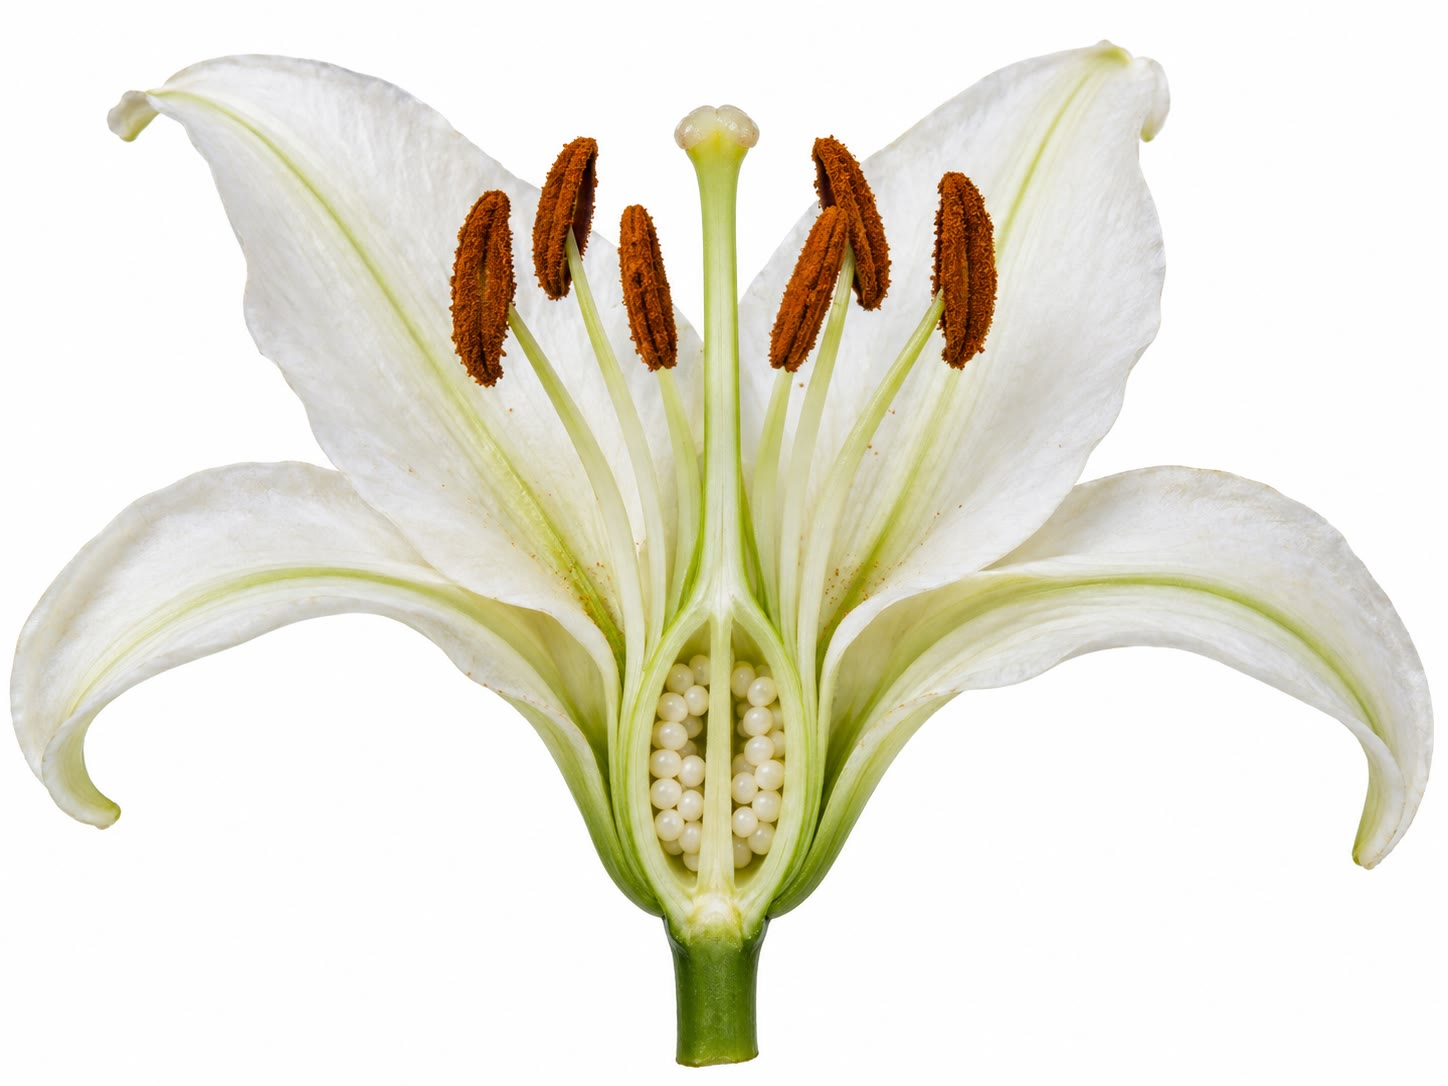
\includegraphics[width=0.55\linewidth]{images/book4/ai/b4-06-lily-dissected.jpg}

{\small Un lis coupé dans le sens de la longueur~: six \omterm{def:b2:angiosperm-reproduction:flower}{étamines} aux
anthères chargées de \omterm{def:b2:plant-life-cycles:heterospory}{pollen}, le long style et son \omterm{def:b2:angiosperm-reproduction:flower}{stigmate} collant, et
l'\omterm{def:b2:angiosperm-reproduction:flower}{ovaire} ouvert montrant les rangées d'\omterm{def:b2:plant-life-cycles:heterospory}{ovules}.}
\end{omfigure}

\section{Les deux gamétophytes}

\begin{proposition}[Le pollen~: le gamétophyte mâle]\label{prop:b2:angiosperm-reproduction:pollen}
\index{grain de pollen}\index{microsporogenese@microsporogenèse}\index{sporopollenine@sporopollénine}
Dans chaque sac pollinique, des cellules mères \omterm{def:b2:meiosis-heredity:meiosis}{diploïdes} subissent la
\omterm{def:b2:meiosis-heredity:meiosis}{méiose} et donnent des tétrades de \emph{\omterm{def:b2:plant-life-cycles:heterospory}{microspores}}. Chaque \omterm{def:b2:plant-life-cycles:heterospory}{microspore}
se divise une fois, de façon inégale, en une grande \emph{cellule
végétative} et une petite \emph{cellule génératrice} incluse dans la
première~; la cellule génératrice se divise encore une fois, avant ou
après la \omterm{def:b2:angiosperm-reproduction:pollination}{pollinisation}, en deux \emph{cellules spermatiques}. Le
\emph{\omterm{prop:b2:angiosperm-reproduction:pollen}{grain de pollen}} mûr est ainsi un organisme \omterm{def:b2:meiosis-heredity:meiosis}{haploïde} de trois
cellules --- le gamétophyte mâle tout entier --- de
\qtyrange{10}{100}{\micro m}, enfermé dans une paroi dont la couche
externe de \emph{sporopollénine}, le polymère biologique le plus
résistant que l'on connaisse, est sculptée d'épines, de pores et de
sillons caractéristiques de l'espèce, ce qui explique que le \omterm{def:b2:plant-life-cycles:heterospory}{pollen}
permette d'identifier des plantes dans des sédiments vieux de dizaines
de millions d'années. Le grain est libéré déshydraté et survit de
quelques heures (graminées) à quelques semaines (certains arbres)
jusqu'à ce qu'il atteigne un \omterm{def:b2:angiosperm-reproduction:flower}{stigmate}.
\end{proposition}

\begin{omfigure}
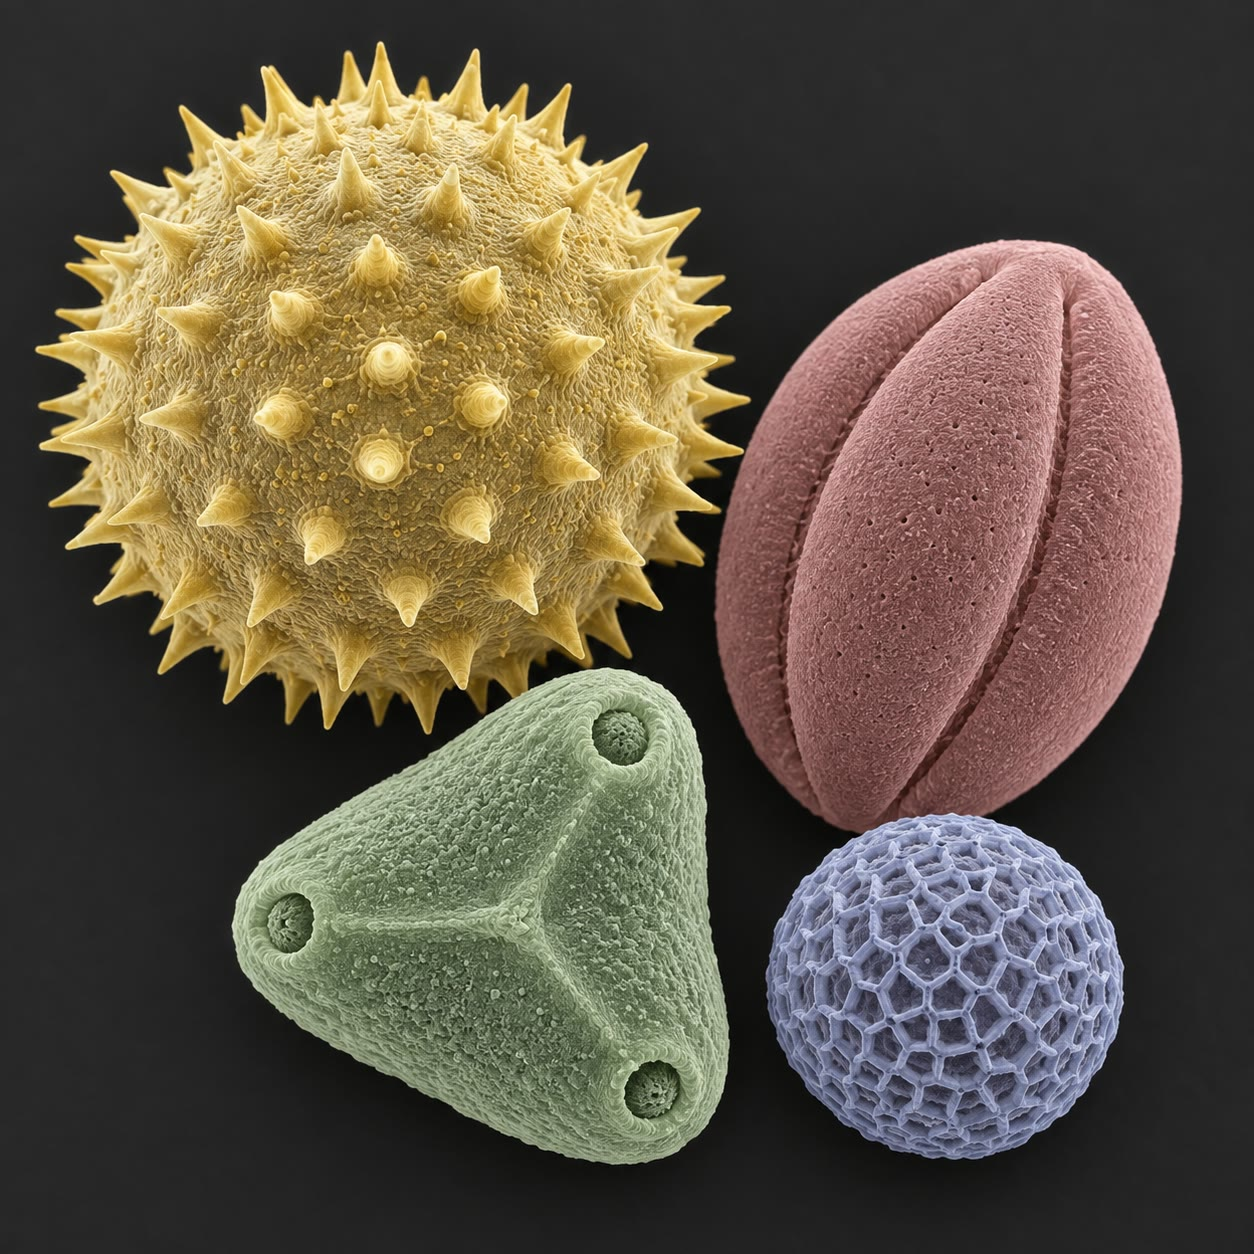
\includegraphics[width=0.45\linewidth]{images/book4/ai/b4-06-pollen-sem.jpg}

{\small \omterm{prop:b2:angiosperm-reproduction:pollen}{Grains de pollen} au microscope électronique à balayage~: la paroi
de sporopollénine de chaque espèce a sa propre ornementation ---
épines, sillons, pores, réseau --- qui permet de la reconnaître.}
\end{omfigure}

\begin{proposition}[Le sac embryonnaire~: le gamétophyte femelle]\label{prop:b2:angiosperm-reproduction:embryosac}
\index{sac embryonnaire}\index{macrosporogenese@macrosporogenèse}\index{noyaux polaires}
Dans chaque \omterm{def:b2:plant-life-cycles:heterospory}{ovule}, une cellule \omterm{def:b2:meiosis-heredity:meiosis}{diploïde} du nucelle subit la \omterm{def:b2:meiosis-heredity:meiosis}{méiose}~;
trois des quatre \omterm{def:b2:plant-life-cycles:heterospory}{macrospores} dégénèrent, et la quatrième se développe,
par trois mitoses sans division cellulaire, en un \emph{\omterm{prop:b2:angiosperm-reproduction:embryosac}{sac
embryonnaire}} à huit noyaux et sept cellules~: du côté du micropyle,
l'\emph{oosphère} flanquée de deux \emph{synergides}~; à l'extrémité
opposée, trois cellules \emph{antipodes}~; au milieu, une grande
\emph{cellule centrale} contenant deux \emph{\omterm{prop:b2:angiosperm-reproduction:embryosac}{noyaux polaires}}. Ce sac,
enveloppé du nucelle et de deux téguments percés d'un micropyle, est
le gamétophyte femelle tout entier --- sept cellules là où une \omterm{def:b2:plant-life-cycles:moss}{mousse}
avait une plante. Les deux \omterm{prop:b2:angiosperm-reproduction:embryosac}{noyaux polaires} sont génétiquement
identiques à l'oosphère, un fait qui compte pour l'albumen.
\end{proposition}

\begin{omfigure}
\begin{tikzpicture}[every node/.style={font=\scriptsize}]
  % pollen grain
  \begin{scope}
    \draw[very thick, omProp!80!black, fill=omProp!15] (0,0) circle (1.1);
    \draw[thick, omProp!80!black] (0,0) circle (0.95);
    \foreach \a in {0,30,...,330} \draw[omProp!80!black, thick] (\a:1.1) -- (\a:1.25);
    \draw[thick, fill=omDef!25] (0.15,-0.2) ellipse (0.55 and 0.4); \node[font=\tiny] at (0.15,-0.2) {végétative};
    \draw[thick, fill=omThm!30] (-0.3,0.45) ellipse (0.22 and 0.14); \draw[thick, fill=omThm!30] (0.2,0.5) ellipse (0.22 and 0.14);
    \draw[omThm] (0.0,0.62) -- (0.0,1.5); \node[omThm, anchor=south] at (0.0,1.5) {deux cellules spermatiques};
    \node[below, align=center] at (0,-1.4) {grain de pollen ($n$)\\3 cellules, paroi de sporopollénine};
  \end{scope}
  % ovule with embryo sac
  \begin{scope}[xshift=5.5cm]
    \draw[thick, fill=omExo!25] (0,0) ellipse (1.5 and 2.1);
    \draw[thick, fill=omExo!10] (0,0) ellipse (1.15 and 1.75);
    \fill[white] (-0.3,1.7) rectangle (0.3,2.2); \draw[thick] (-0.3,1.7) -- (-0.3,2.15); \draw[thick] (0.3,1.7) -- (0.3,2.15);
    \draw[thick, fill=white] (0,0) ellipse (0.7 and 1.35);
    % cells: egg + synergids top, central, antipodals bottom
    \draw[thick, fill=omThm!30] (0,0.95) circle (0.17); \node[omThm, anchor=west] at (1.6,1.2) {oosphère};
    \draw[thick, fill=omDef!25] (-0.35,1.0) circle (0.14); \draw[thick, fill=omDef!25] (0.35,1.0) circle (0.14); \node[anchor=west] at (1.6,0.75) {deux synergides};
    \draw[thick, fill=omDef!10] (0,0) ellipse (0.55 and 0.6); \fill[omDef!80!black] (-0.15,0.05) circle (0.09); \fill[omDef!80!black] (0.15,0.05) circle (0.09);
    \node[anchor=west, align=left] at (1.6,0.1) {cellule centrale à\\deux noyaux polaires};
    \foreach \x in {-0.3,0,0.3} \draw[thick, fill=omDef!25] (\x,-1.0) circle (0.13); \node[anchor=west] at (1.6,-1.0) {trois antipodes};
    \draw (0.35,2.0) -- (1.6,2.0) node[right] {micropyle};
    \draw (1.3,-0.9) -- (1.6,-1.6) node[right] {téguments};
    \draw (0.9,-1.35) -- (1.6,-2.1) node[right] {nucelle};
    \draw (1.6,1.2) -- (0.17,0.95); \draw (1.6,0.75) -- (0.49,1.0); \draw (1.6,0.1) -- (0.55,0.05); \draw (1.6,-1.0) -- (0.43,-1.0);
    \node[below, align=center] at (0,-2.3) {ovule et sac embryonnaire ($n$)\\7 cellules, 8 noyaux};
  \end{scope}
\end{tikzpicture}

{\small Les deux gamétophytes d'une plante à \omterm{def:b2:angiosperm-reproduction:flower}{fleurs}, tous deux réduits à
quelques cellules~: le \omterm{prop:b2:angiosperm-reproduction:pollen}{grain de pollen} à trois cellules, et le \omterm{prop:b2:angiosperm-reproduction:embryosac}{sac
embryonnaire} à sept cellules à l'intérieur de l'\omterm{def:b2:plant-life-cycles:heterospory}{ovule}.}
\end{omfigure}

\section{La pollinisation}

\begin{definition}[La pollinisation et ses agents]\label{def:b2:angiosperm-reproduction:pollination}
\index{pollinisation}\index{syndrome de pollinisation}\index{nectar}
La \emph{pollinisation} est le transport du \omterm{def:b2:plant-life-cycles:heterospory}{pollen} d'une anthère à un
\omterm{def:b2:angiosperm-reproduction:flower}{stigmate}~; l'\emph{autopollinisation} a lieu au sein d'une même \omterm{def:b2:angiosperm-reproduction:flower}{fleur}
ou d'une même plante, la \emph{pollinisation croisée} entre plantes
différentes. Les \omterm{def:b2:angiosperm-reproduction:flower}{fleurs} \emph{anémophiles} (graminées, chênes, bouleaux,
plantains) sont petites, vertes, sans parfum, avec de grands \omterm{def:b2:angiosperm-reproduction:flower}{stigmates}
plumeux et d'énormes quantités de \omterm{def:b2:plant-life-cycles:heterospory}{pollen} lisse et sec~; leur rapport
\omterm{def:b2:plant-life-cycles:heterospory}{pollen}/\omterm{def:b2:plant-life-cycles:heterospory}{ovule} atteint le million. Les \omterm{def:b2:angiosperm-reproduction:flower}{fleurs} \emph{zoophiles}
rétribuent leur transporteur~: \emph{nectar} (solution sucrée sécrétée
par des nectaires), \omterm{def:b2:plant-life-cycles:heterospory}{pollen} lui-même, huiles, parfum~; et elles
signalent leur présence par une couleur, une forme et une odeur
accordées aux sens du transporteur --- guides à nectar ultraviolets pour
les abeilles, qui voient l'ultraviolet mais pas le rouge~; \omterm{def:b2:angiosperm-reproduction:flower}{fleurs}
rouges tubulaires et sans parfum pour les colibris~; \omterm{def:b2:angiosperm-reproduction:flower}{fleurs} blanches,
très parfumées, s'ouvrant la nuit et à tube profond pour les
papillons de nuit~; \omterm{def:b2:angiosperm-reproduction:flower}{fleurs} brunes et fétides pour les mouches
nécrophages~; \omterm{def:b2:angiosperm-reproduction:flower}{fleurs} robustes, pâles et nocturnes pour les chauves-souris.
Chacun de ces ensembles de caractères est un \emph{syndrome de
pollinisation}, et l'ajustement entre la \omterm{def:b2:angiosperm-reproduction:flower}{fleur} et son pollinisateur est
le cas d'école de la \emph{coévolution}~: à partir de l'éperon
nectarifère de \qty{30}{cm} d'une orchidée de Madagascar, Darwin
prédit un papillon de nuit à trompe de \qty{30}{cm}, découvert quarante
ans plus tard.
\end{definition}

\begin{omfigure}
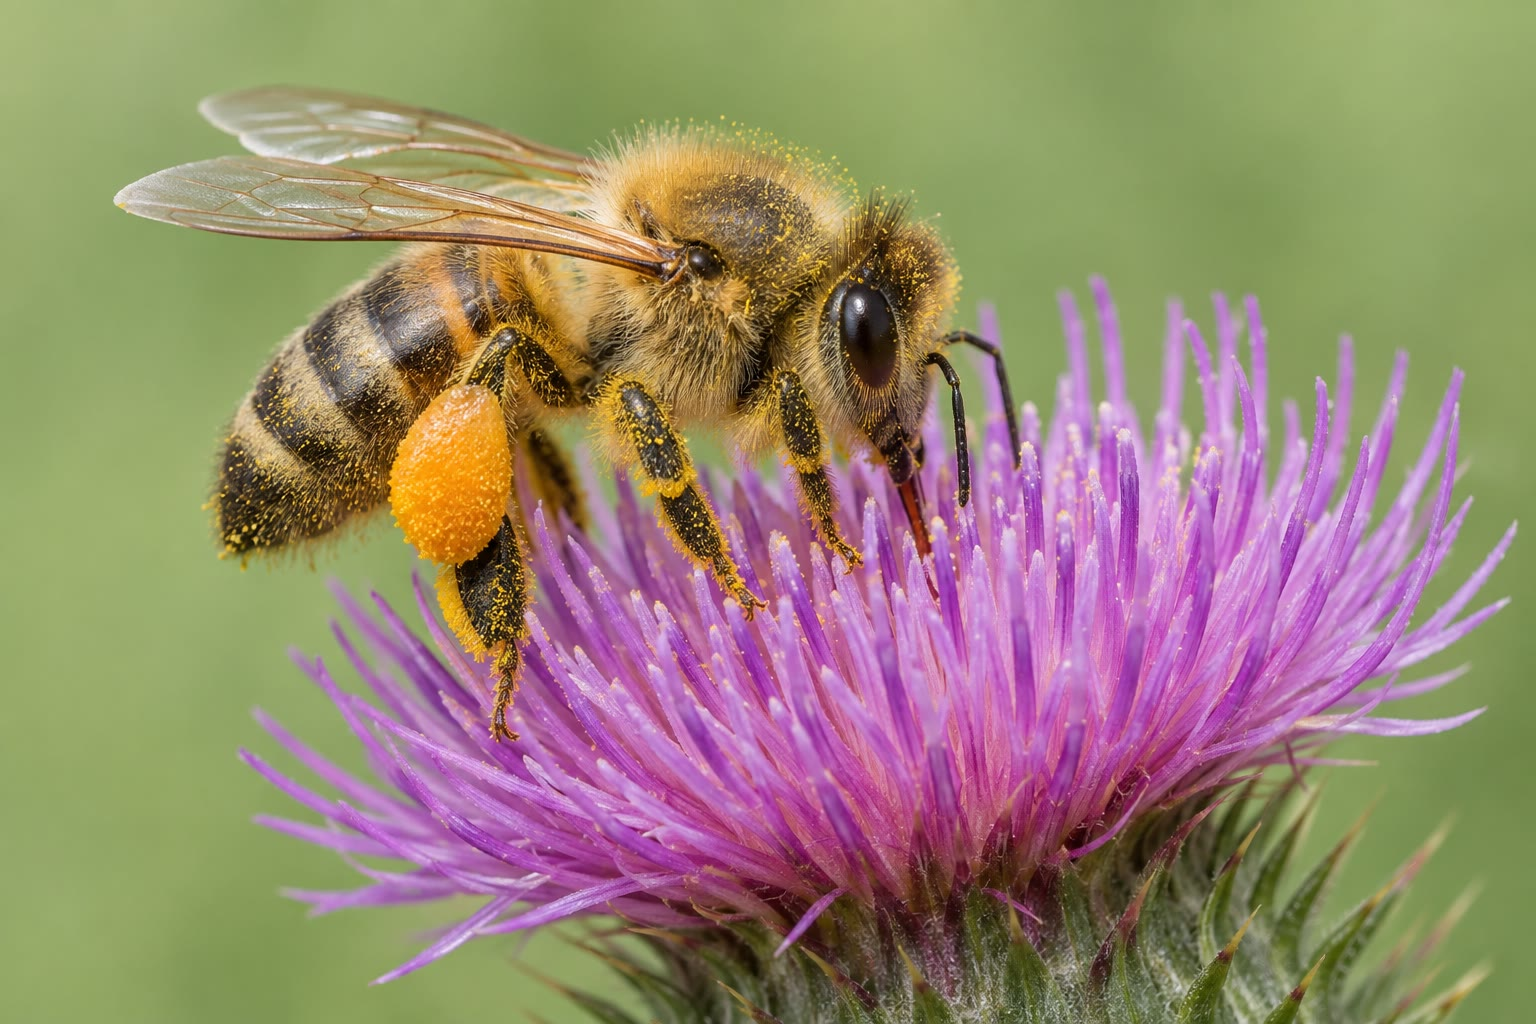
\includegraphics[width=0.58\linewidth]{images/book4/ai/b4-06-bee-on-flower.jpg}

{\small Une abeille domestique sur un chardon~: le \omterm{def:b2:plant-life-cycles:heterospory}{pollen} saupoudre son
corps et s'entasse dans les corbeilles de ses pattes postérieures~; une
partie atteindra le \omterm{def:b2:angiosperm-reproduction:flower}{stigmate} du prochain chardon visité. Couleur
pourpre, piste d'atterrissage et \omterm{def:b2:angiosperm-reproduction:pollination}{nectar} abondant forment le syndrome de
l'abeille.}
\end{omfigure}

\begin{proposition}[Éviter l'autofécondation]\label{prop:b2:angiosperm-reproduction:selfing}
\index{auto-incompatibilite@auto-incompatibilité}\index{heterostylie@hétérostylie}\index{dichogamie}
Une \omterm{def:b2:angiosperm-reproduction:flower}{fleur} hermaphrodite pourrait se féconder elle-même, et beaucoup le
font (pois, blé, tomate)~; mais l'autofécondation expose les \omterm{def:b2:meiosis-heredity:vocabulary}{allèles}
\omterm{def:b2:meiosis-heredity:vocabulary}{récessifs} délétères (\emph{dépression de consanguinité}), et la
plupart des espèces l'empêchent. Dans le temps~: la \emph{dichogamie},
maturation des anthères et du \omterm{def:b2:angiosperm-reproduction:flower}{stigmate} à des moments différents
(protandrie chez la plupart des ombellifères et des composées). Dans
l'espace~: l'\emph{herkogamie}, anthères et \omterm{def:b2:angiosperm-reproduction:flower}{stigmate} tenus à distance,
comme dans l'\emph{hétérostylie} des primevères, dont les \omterm{def:b2:angiosperm-reproduction:flower}{fleurs}
longistylées (style long, anthères basses) et brévistylées (style
court, anthères hautes) déposent le \omterm{def:b2:plant-life-cycles:heterospory}{pollen} sur des parties différentes
d'un insecte. Par la biochimie~: l'\emph{auto-incompatibilité}, un
système de reconnaissance dans lequel le \omterm{def:b2:plant-life-cycles:heterospory}{pollen} porteur d'un \omterm{def:b2:meiosis-heredity:vocabulary}{allèle} $S$
commun avec le pistil est rejeté. Dans l'incompatibilité
\emph{gamétophytique} (pommier, cerisier, pétunia, graminées), c'est
l'\omterm{def:b2:meiosis-heredity:vocabulary}{allèle} $S$ \omterm{def:b2:meiosis-heredity:meiosis}{haploïde} du \omterm{def:b2:plant-life-cycles:heterospory}{pollen} lui-même qui décide~: un pistil
$S_1S_2$ arrête dans le style les tubes $S_1$ et $S_2$, si bien que le
\omterm{def:b2:plant-life-cycles:heterospory}{pollen} d'une plante $S_1S_3$ est compatible pour moitié et celui d'une
plante $S_3S_4$ entièrement. Dans l'incompatibilité
\emph{sporophytique} (chou, tournesol), c'est le \omterm{def:b2:meiosis-heredity:vocabulary}{génotype} \omterm{def:b2:meiosis-heredity:meiosis}{diploïde} de la
plante qui a produit le \omterm{def:b2:plant-life-cycles:heterospory}{pollen} qui décide, à la surface du \omterm{def:b2:angiosperm-reproduction:flower}{stigmate}. Un
\omterm{def:b2:meiosis-heredity:vocabulary}{allèle} $S$ rare est compatible avec presque tous les partenaires~: la
sélection maintient donc des dizaines d'\omterm{def:b2:meiosis-heredity:vocabulary}{allèles} dans une population.
\end{proposition}
\begin{proof}[Faits expérimentaux]
Darwin (1862, 1877) croisa des primevères à la main~: le \omterm{def:b2:plant-life-cycles:heterospory}{pollen} d'une
\omterm{def:b2:angiosperm-reproduction:flower}{fleur} brévistylée déposé sur un \omterm{def:b2:angiosperm-reproduction:flower}{stigmate} longistylé (une union
«~légitime~») donnait des capsules pleines~; longistylée sur longistylée
ou brévistylée sur brévistylée («~illégitime~») donnait peu de \omterm{def:b2:angiosperm-reproduction:seed}{graines}
ou aucune, bien que les plantes fussent saines et le \omterm{def:b2:plant-life-cycles:heterospory}{pollen} vivant. Il
en conclut que les deux formes étaient adaptées l'une à l'autre pour se
croiser et protégées de l'autofécondation et, en comptant les \omterm{def:b2:angiosperm-reproduction:seed}{graines}
par capsule dans des milliers de croisements, il mesura le coût de
l'autofécondation chez des dizaines d'espèces~: les descendants
autofécondés étaient plus petits, plus légers et moins fertiles,
génération après génération.
\end{proof}

\begin{omfigure}
\begin{tikzpicture}[every node/.style={font=\scriptsize}]
  % pistil S1S2 with pollen tubes
  \draw[thick, fill=omDef!10] (-0.5,0) rectangle (0.5,3.2);
  \draw[thick, fill=omDef!30] (0,3.3) ellipse (0.7 and 0.2);
  \draw[thick, fill=omDef!12] (0,-0.6) ellipse (0.9 and 0.7);
  \node at (0,-0.6) {ovaire};
  \node[anchor=east] at (-1.1,3.3) {stigmate d'une plante $S_1S_2$};
  % pollen grains
  \draw[thick, fill=omThm!40] (-0.35,3.75) circle (0.13); \node[omThm, left] at (-0.5,3.75) {$S_1$};
  \draw[thick, fill=omThm!40] (0,3.75) circle (0.13); \node[omThm, anchor=south] at (0,3.92) {$S_2$};
  \draw[thick, fill=omExo!70!black] (0.35,3.75) circle (0.13); \node[right] at (0.5,3.75) {$S_3$};
  % tubes: S1 and S2 stop in the style, S3 reaches the ovary
  \draw[thick, omThm] (-0.35,3.3) -- (-0.35,2.3); \node[omThm, left, align=right] at (-0.55,2.3) {tube $S_1$\\arrêté};
  \draw[thick, omThm] (0,3.3) -- (0,2.0);
  \draw[thick, omExo!70!black] (0.35,3.3) -- (0.35,-0.2) -- (0.2,-0.5);
  \node[right, align=left] at (0.55,0.9) {le tube $S_3$\\atteint un ovule};
  \node[anchor=west, align=left, text width=6cm] at (3.2,3.2) {auto-incompatibilité gamétophytique~: un tube pollinique dont l'allèle $S$ est identique à l'un des allèles du pistil est arrêté dans le style};
  \node[anchor=west, align=left, text width=6cm] at (3.2,1.4) {pollen d'une plante $S_1S_2$~: 0 compatible\\d'une plante $S_1S_3$~: moitié\\d'une plante $S_3S_4$~: tout};
\end{tikzpicture}

{\small L'auto-incompatibilité gamétophytique. Sur un pistil $S_1S_2$,
les tubes portant $S_1$ ou $S_2$ sont arrêtés dans le style~; un tube
$S_3$ croît jusqu'à l'\omterm{def:b2:angiosperm-reproduction:flower}{ovaire}.}
\end{omfigure}

\section{La fécondation}

\begin{theorem}[Le tube pollinique]\label{thm:b2:angiosperm-reproduction:tube}
\index{tube pollinique}
Un \omterm{prop:b2:angiosperm-reproduction:pollen}{grain de pollen} déposé sur un \omterm{def:b2:angiosperm-reproduction:flower}{stigmate} compatible se réhydrate et
émet un \emph{\omterm{thm:b2:angiosperm-reproduction:tube}{tube pollinique}}~: la cellule végétative s'allonge par
croissance apicale, en déposant une paroi nouvelle à l'apex à raison de
\qtyrange{0.1}{1}{cm/h}, en se frayant un chemin par digestion à
travers le tissu de transmission du style et en s'en nourrissant. Le
tube transporte les deux cellules spermatiques à son extrémité~; il est
guidé sur la dernière distance par des peptides sécrétés par les
synergides, entre dans l'\omterm{def:b2:plant-life-cycles:heterospory}{ovule} par le micropyle, éclate dans une
synergide et libère les cellules spermatiques. Un tube qui traverse un
style de longueur $L$ à la vitesse $v$ met un temps $L/v$~: quelques
heures chez le cerisier, une journée entière chez le maïs, dont les
«~soies~» sont des styles de \qty{20}{cm}. La viabilité du \omterm{def:b2:plant-life-cycles:heterospory}{pollen}
impose un compte à rebours~: le \omterm{def:b2:plant-life-cycles:heterospory}{pollen} des graminées meurt en quelques
heures, si bien qu'un \omterm{def:b2:angiosperm-reproduction:flower}{stigmate} doit être atteint rapidement.
\end{theorem}
\begin{proof}
Le temps est la longueur divisée par la vitesse de croissance~; pour le
maïs, \qty{20}{cm} à \qty{1}{cm/h} donnent \qty{20}{h}. Le tube
lui-même est presque entièrement fait de paroi et d'une mince pellicule
de cytoplasme derrière l'apex, si bien que les réserves de la cellule
végétative, augmentées de ce qu'elle absorbe dans le style, suffisent
pour une longueur mille fois supérieure au diamètre du grain.
\end{proof}

\begin{proposition}[La double fécondation]\label{prop:b2:angiosperm-reproduction:double}
\index{double fecondation@double fécondation}\index{albumen}
Des deux cellules spermatiques délivrées par le tube, l'une fusionne
avec l'oosphère pour former le \emph{zygote} \omterm{def:b2:meiosis-heredity:meiosis}{diploïde}, d'où se
développe l'embryon~; l'autre fusionne avec la cellule centrale et ses
deux \omterm{prop:b2:angiosperm-reproduction:embryosac}{noyaux polaires} pour former un noyau \emph{triploïde} ($3n$~: deux
génomes maternels, un paternel), d'où se développe l'\emph{albumen}
--- un tissu nutritif qui remplit la \omterm{def:b2:angiosperm-reproduction:seed}{graine} d'amidon, d'huile et de
protéines. Les deux fécondations ont lieu à quelques minutes
d'intervalle~; chez la plupart des espèces, aucune ne réussit sans
l'autre, si bien qu'une plante n'approvisionne que les \omterm{def:b2:angiosperm-reproduction:seed}{graines} qui
portent un embryon. L'albumen est le tissu qui nourrit l'humanité~: la
farine du blé et du riz, la semoule du maïs, la chair blanche de la noix
de coco sont de l'albumen triploïde. Chez les gymnospermes, la réserve
de la \omterm{def:b2:angiosperm-reproduction:seed}{graine} est le gamétophyte femelle, construit avant la fécondation,
qu'un embryon suive ou non~; l'albumen des angiospermes est fait sur
commande.
\end{proposition}
\begin{proof}[Faits expérimentaux]
Nawaschin (1898), suivant au microscope le \omterm{thm:b2:angiosperm-reproduction:tube}{tube pollinique} d'un lis et
d'une fritillaire jusque dans le \omterm{prop:b2:angiosperm-reproduction:embryosac}{sac embryonnaire}, vit les deux noyaux
spermatiques quitter le tube, l'un entrant dans l'oosphère et l'autre
fusionnant avec les \omterm{prop:b2:angiosperm-reproduction:embryosac}{noyaux polaires}~; Guignard le confirma l'année
suivante chez d'autres espèces. La triploïdie de l'albumen découla des
dénombrements de chromosomes, et ses conséquences génétiques --- un
albumen de grain montrant les caractères du parent pollinisateur
(\emph{xénie}), dans le rapport de deux doses maternelles pour une dose
paternelle --- avaient été remarquées bien auparavant par les
sélectionneurs de maïs.
\end{proof}

\begin{omfigure}
\begin{tikzpicture}[every node/.style={font=\scriptsize}, >=stealth]
  \node[draw, rounded corners, fill=omProp!15, align=center] (sp) at (0,2) {cellule spermatique 1 ($n$)};
  \node[draw, rounded corners, fill=omProp!15, align=center] (sp2) at (0,0) {cellule spermatique 2 ($n$)};
  \node[draw, rounded corners, fill=omThm!15, align=center] (egg) at (4,2) {oosphère ($n$)};
  \node[draw, rounded corners, fill=omDef!15, align=center] (cc) at (4,0) {cellule centrale\\deux noyaux polaires ($n + n$)};
  \node[draw, rounded corners, fill=omThm!30, align=center] (zyg) at (8.6,2) {zygote ($2n$)\\$\to$ embryon};
  \node[draw, rounded corners, fill=omDef!30, align=center] (endo) at (8.6,0) {noyau de l'albumen ($3n$)\\$\to$ albumen, la réserve nutritive};
  \draw[->, thick] (sp) -- (egg); \draw[->, thick] (egg) -- (zyg);
  \draw[->, thick] (sp2) -- (cc); \draw[->, thick] (cc) -- (endo);
  \node[anchor=south] at (2,2.5) {fécondation 1};
  \node[anchor=south] at (2,0.5) {fécondation 2};
  \node[anchor=north, align=center] at (4.3,-0.9) {un tube pollinique, deux cellules spermatiques, deux fusions~: l'embryon et sa réserve sont produits ensemble};
\end{tikzpicture}

{\small La \omterm{prop:b2:angiosperm-reproduction:double}{double fécondation}~: une cellule spermatique produit le
zygote \omterm{def:b2:meiosis-heredity:meiosis}{diploïde}, l'autre l'albumen triploïde.}
\end{omfigure}

\section{Graine et fruit}

\begin{definition}[De l'ovule à la graine, de l'ovaire au fruit]\label{def:b2:angiosperm-reproduction:seed}
\index{graine}\index{fruit}\index{cotyledon@cotylédon}\index{dormance}
Le zygote se divise en un suspenseur, qui enfonce l'embryon dans
l'albumen, et un embryon proprement dit qui passe par les stades
globulaire, cordiforme et torpille tout en établissant les pôles
racinaire et caulinaire et un ou deux \emph{cotylédons} (feuilles
embryonnaires) --- la distinction entre monocotylédones et
dicotylédones. Chez de nombreuses dicotylédones (haricot, pois), les
cotylédons en croissance absorbent l'albumen et deviennent eux-mêmes la
réserve~; chez les céréales et la plupart des monocotylédones,
l'albumen persiste et le cotylédon unique est un organe suceur. Les
téguments durcissent en \emph{tégument de la graine}~; la graine se
déshydrate jusqu'à \qtyrange{5}{15}{\%} d'eau, le métabolisme
s'arrête, et elle entre en \emph{dormance}, qui ne prend fin que
lorsqu'un signal --- l'eau, le froid, la lumière, le feu, le passage
dans un tube digestif --- indique que la saison est favorable.
Pendant ce temps, la paroi de l'\omterm{def:b2:angiosperm-reproduction:flower}{ovaire} se développe en \emph{fruit},
dont la forme est une stratégie de dispersion~: fruits secs qui
s'ouvrent (gousses, capsules) ou non (caryopses, noix, samares ailées),
fruits charnus qui sont mangés (baies, drupes à noyau, la pomme, dont la
chair est le réceptacle)~; la graine traverse l'animal sans dommage, son
tégument scarifié, et se trouve déposée avec de l'engrais à des
kilomètres de là.
\end{definition}
\begin{proof}[Faits expérimentaux]
Le grain de céréale montre comment la germination est contrôlée.
L'embryon, en s'imbibant d'eau, sécrète de la gibbérelline dans
l'albumen qui l'entoure~; la couche externe de l'albumen, la couche à
aleurone, répond en fabriquant et en sécrétant de l'$\alpha$-amylase,
qui digère l'amidon en sucres que l'embryon absorbe. Des demi-grains
dépourvus d'embryon ne fabriquent pas d'amylase~; si on leur ajoute de
la gibbérelline, ils en fabriquent (Paleg, Yomo, 1960)~; l'hormone agit
en activant le gène de l'amylase, l'un des premiers cas où une hormone
végétale fut reliée à un gène. Les brasseurs utilisent ce processus
depuis des millénaires~: le maltage consiste à faire germer l'orge puis
à la sécher.
\end{proof}

\begin{omfigure}
\begin{tikzpicture}[every node/.style={font=\scriptsize}]
  % embryogenesis stages
  \foreach \x/\lab in {0/{zygote}, 1.6/{deux cellules}, 3.4/{globulaire}, 5.6/{cordiforme}, 8.2/{torpille}} \node[below] at (\x,-1.1) {\lab};
  \draw[thick, fill=omThm!25] (0,-0.2) circle (0.22);
  \draw[thick, fill=omThm!25] (1.6,0.0) circle (0.2); \draw[thick, fill=omDef!15] (1.6,-0.45) circle (0.14);
  \draw[thick, fill=omThm!25] (3.4,0.1) circle (0.45); \foreach \y in {-0.5,-0.75,-1.0} \draw[thick, fill=omDef!15] (3.4,\y) circle (0.1);
  \draw[thick, fill=omThm!25] (5.6,0.0) .. controls (4.9,1.0) and (5.2,-0.6) .. (5.6,-0.6) .. controls (6.0,-0.6) and (6.3,1.0) .. (5.6,0.0);
  \draw[thick, fill=omThm!25] (5.15,0.5) circle (0.32); \draw[thick, fill=omThm!25] (6.05,0.5) circle (0.32);
  \foreach \y in {-0.75,-1.0} \draw[thick, fill=omDef!15] (5.6,\y) circle (0.09);
  \draw[thick, fill=omThm!25] (8.2,-0.2) ellipse (0.3 and 0.75);
  \draw[thick, fill=omThm!25] (7.75,0.9) .. controls (7.4,1.6) and (7.9,1.9) .. (8.05,0.55) -- cycle;
  \draw[thick, fill=omThm!25] (8.65,0.9) .. controls (9.0,1.6) and (8.5,1.9) .. (8.35,0.55) -- cycle;
  \node[omDef!80!black, anchor=west] at (9.3,-0.9) {suspenseur (en bleu)};
  \node[omThm, anchor=west] at (9.3,0.9) {cotylédons};
  \node[anchor=west] at (9.3,-0.2) {pôle racinaire en bas};
\end{tikzpicture}

{\small L'embryogenèse chez une dicotylédone~: le zygote se divise en un
embryon et un suspenseur~; l'embryon globulaire devient cordiforme à
mesure qu'émergent les deux \omterm{def:b2:angiosperm-reproduction:seed}{cotylédons}, puis prend la forme d'une
torpille à mesure que s'allonge l'axe racine--tige.}
\end{omfigure}

\begin{omfigure}
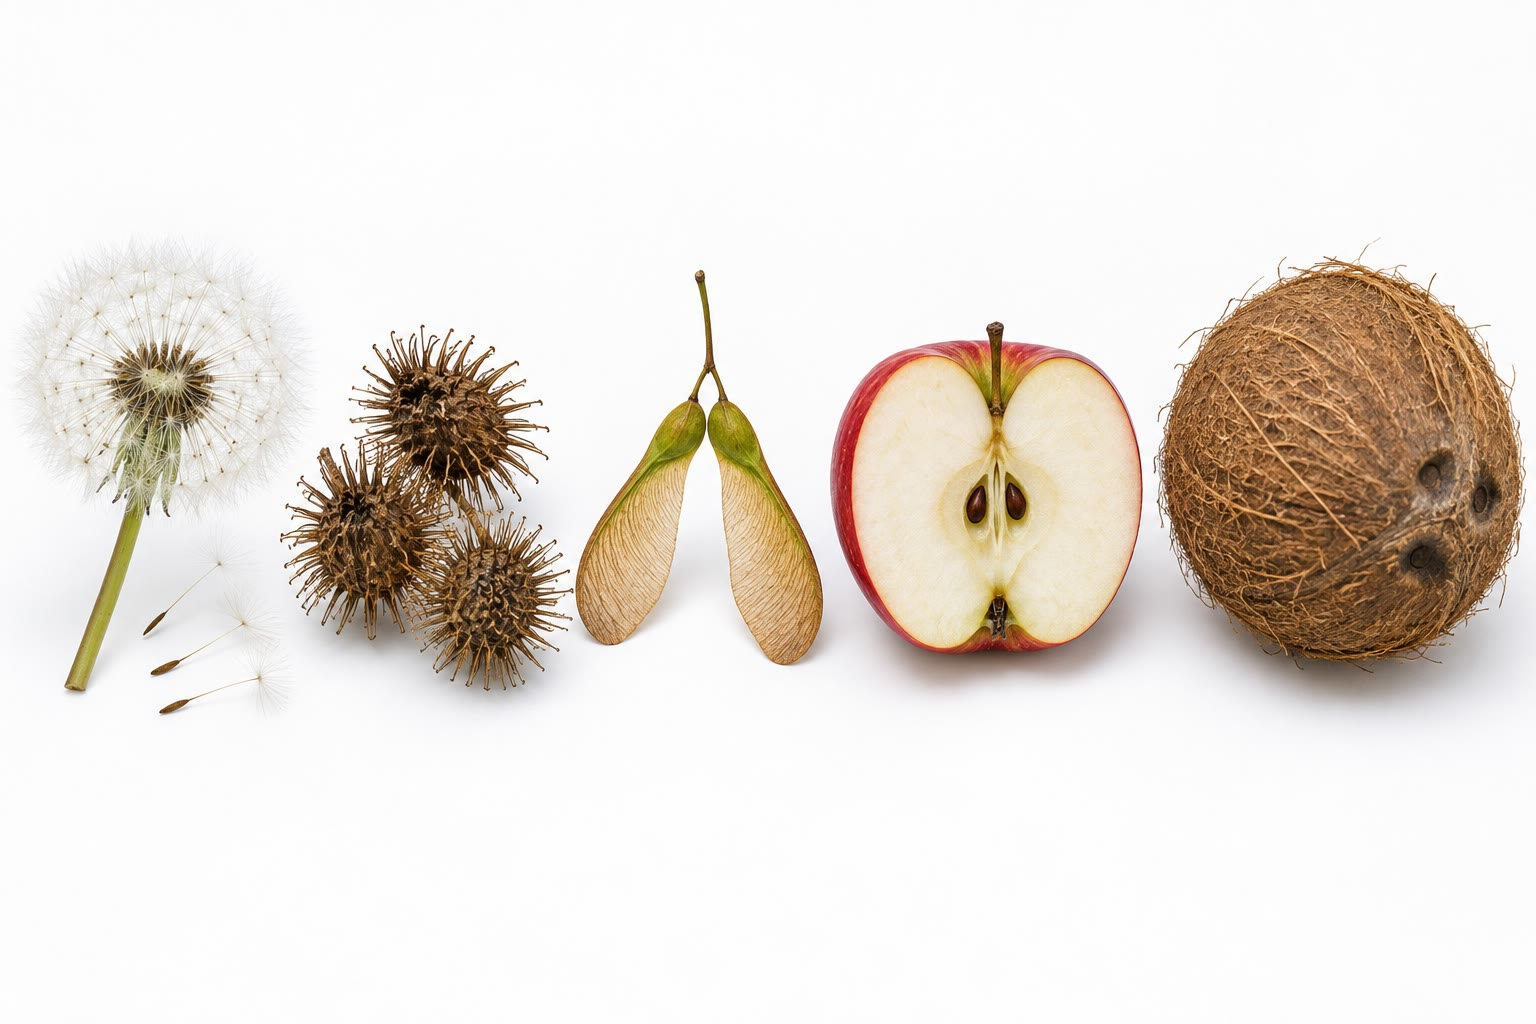
\includegraphics[width=0.62\linewidth]{images/book4/ai/b4-06-fruits-seeds.jpg}

{\small Des \omterm{def:b2:angiosperm-reproduction:seed}{fruits} faits pour la dispersion~: parachutes (pissenlit),
crochets (bardane), ailes (érable), chair offerte à un animal (pomme),
et bourre flottante pour la mer (noix de coco).}
\end{omfigure}

\begin{example}[Distances de dispersion]\label{ex:b2:angiosperm-reproduction:dispersal}
Un akène de pissenlit muni de son parachute descend à \qty{0.3}{m/s}~;
libéré à \qty{0.3}{m} dans un vent de \qty{3}{m/s}, il vole \qty{3}{m},
et dans une ascendance thermique, des centaines. Une samare d'érable
descend en autorotation à \qty{1}{m/s} depuis \qty{15}{m}~:
\qty{45}{m}. Un noyau de cerise lâché par un oiseau après un vol de
vingt minutes à \qty{10}{m/s}~: jusqu'à \qty{12}{km}. Les glands d'un
chêne tombent à son pied, à moins qu'un geai ne les emporte, ce qu'il
fait par milliers, à un kilomètre et plus, en oubliant un dixième
d'entre eux~: les chênes qui recolonisèrent l'Europe après la dernière
glaciation remontèrent vers le nord à des centaines de mètres par an,
bien plus vite qu'un gland ne roule, et ce sont les oiseaux qui les ont
déplacés.
\end{example}

\section{Exercices}

\begin{exercise}[$\star$]\label{exo:b2:angiosperm-reproduction:1}
Nommer les quatre verticilles d'une \omterm{def:b2:angiosperm-reproduction:flower}{fleur}, ainsi que les parties d'une
\omterm{def:b2:angiosperm-reproduction:flower}{étamine} et d'un \omterm{def:b2:angiosperm-reproduction:flower}{carpelle}. Quelles parties appartiennent au \omterm{def:b2:plant-life-cycles:cycles}{sporophyte}
\omterm{def:b2:meiosis-heredity:meiosis}{diploïde}, lesquelles au gamétophyte \omterm{def:b2:meiosis-heredity:meiosis}{haploïde}~?
\end{exercise}

\begin{exercise}[$\star$]\label{exo:b2:angiosperm-reproduction:2}
Donner la ploïdie~: d'une \omterm{def:b2:plant-life-cycles:heterospory}{microspore}, de la cellule végétative, d'une
cellule spermatique, de l'oosphère, d'un noyau polaire, du zygote, de
l'albumen, du \omterm{def:b2:angiosperm-reproduction:seed}{tégument de la graine}, de la paroi du \omterm{def:b2:angiosperm-reproduction:seed}{fruit}.
\end{exercise}

\begin{exercise}[$\star$]\label{exo:b2:angiosperm-reproduction:3}
Énumérer cinq caractères d'une \omterm{def:b2:angiosperm-reproduction:flower}{fleur} anémophile et cinq d'une \omterm{def:b2:angiosperm-reproduction:flower}{fleur}
pollinisée par les abeilles, et donner une plante pour chacune.
\end{exercise}

\begin{exercise}[$\star$]\label{exo:b2:angiosperm-reproduction:4}
Qu'est-ce que la \omterm{prop:b2:angiosperm-reproduction:double}{double fécondation}, et que produit chacune des deux
fusions~? Pourquoi peut-on dire que l'albumen est «~fait sur
commande~»~?
\end{exercise}

\begin{exercise}[$\star\star$]\label{exo:b2:angiosperm-reproduction:5}
Une soie de maïs mesure \qty{25}{cm} et un \omterm{thm:b2:angiosperm-reproduction:tube}{tube pollinique} croît à
\qty{1.2}{cm/h}. Combien de temps s'écoule entre la \omterm{def:b2:angiosperm-reproduction:pollination}{pollinisation} et la
fécondation~? Une panicule libère du \omterm{def:b2:plant-life-cycles:heterospory}{pollen} du jour 0 au jour 7, et les
soies de la plante émergent du jour 5 au jour 12, un huitième d'entre
elles chaque jour~; une soie ne capte du \omterm{def:b2:plant-life-cycles:heterospory}{pollen} que pendant que le
\omterm{def:b2:plant-life-cycles:heterospory}{pollen} est libéré. Quelle fraction des soies est pollinisée~?
\end{exercise}

\begin{exercise}[$\star\star$]\label{exo:b2:angiosperm-reproduction:6}
Dans le cas d'une auto-incompatibilité gamétophytique, quelle fraction
du \omterm{def:b2:plant-life-cycles:heterospory}{pollen} est compatible dans les croisements $S_1S_2\times S_1S_2$,
$S_1S_2\times
S_1S_3$, $S_1S_2\times S_3S_4$ (le pistil étant indiqué en premier)~?
Donner les \omterm{def:b2:meiosis-heredity:vocabulary}{génotypes} des descendants du deuxième croisement.
\end{exercise}

\begin{exercise}[$\star\star$]\label{exo:b2:angiosperm-reproduction:7}
Dans une population comptant $n$ \omterm{def:b2:meiosis-heredity:vocabulary}{allèles} $S$ de même fréquence, quelle
fraction du \omterm{def:b2:plant-life-cycles:heterospory}{pollen} pris au hasard est compatible avec une plante
donnée~? Expliquer pourquoi un nouvel \omterm{def:b2:meiosis-heredity:vocabulary}{allèle} $S$ apparu par \omterm{def:b2:genome-diversification:mutation}{mutation} se
répand, et ce que cela prédit sur le nombre d'\omterm{def:b2:meiosis-heredity:vocabulary}{allèles}.
\end{exercise}

\begin{exercise}[$\star\star$]\label{exo:b2:angiosperm-reproduction:8}
Une plante de maïs \omterm{def:b2:meiosis-heredity:vocabulary}{hétérozygote} $Yy$ (albumen jaune \omterm{def:b2:meiosis-heredity:vocabulary}{dominant}) est
autofécondée. Donner les \omterm{def:b2:meiosis-heredity:vocabulary}{génotypes} de l'albumen de ses grains et leurs
proportions, en se rappelant que les deux \omterm{prop:b2:angiosperm-reproduction:embryosac}{noyaux polaires} sont
identiques. Quelle fraction des grains est jaune~? Qu'en est-il si la
plante est pollinisée par une plante $yy$~?
\end{exercise}

\begin{exercise}[$\star\star$]\label{exo:b2:angiosperm-reproduction:9}
Décrire l'expérience de la couche à aleurone et expliquer ce qu'elle
montre sur (a) le rôle de l'embryon, (b) le rôle de la gibbérelline,
(c) le lieu de synthèse de l'amylase. Pourquoi le demi-grain sans
embryon est-il le témoin essentiel~?
\end{exercise}

\begin{exercise}[$\star\star\star$]\label{exo:b2:angiosperm-reproduction:10}
Comparer le coût des stratégies anémophile et zoophile~: une plante
anémophile produit $10^{6}$ grains par \omterm{def:b2:plant-life-cycles:heterospory}{ovule}, à \qty{1}{\micro g}
chacun~; une plante zoophile produit $10^{3}$ grains par \omterm{def:b2:plant-life-cycles:heterospory}{ovule}, à
\qty{1}{\micro g} chacun, plus \qty{5}{mg} de sucre de \omterm{def:b2:angiosperm-reproduction:pollination}{nectar} par \omterm{def:b2:angiosperm-reproduction:flower}{fleur}
de dix \omterm{def:b2:plant-life-cycles:heterospory}{ovules}. Calculer le coût reproductif par \omterm{def:b2:plant-life-cycles:heterospory}{ovule} dans chaque cas
(en prenant la même énergie par gramme pour le \omterm{def:b2:plant-life-cycles:heterospory}{pollen} et le sucre), et
expliquer pourquoi la \omterm{def:b2:angiosperm-reproduction:pollination}{pollinisation} par le vent persiste néanmoins.
\end{exercise}

\begin{exercise}[$\star\star\star$]\label{exo:b2:angiosperm-reproduction:11}
Expliquer, à l'aide des chiffres de \cref{ex:b2:angiosperm-reproduction:dispersal},
pourquoi un \omterm{def:b2:angiosperm-reproduction:seed}{fruit} charnu vaut son coût pour un arbre, bien que l'animal
digère la chair et laisse tomber la plupart des \omterm{def:b2:angiosperm-reproduction:seed}{graines} là où elles ne
peuvent pas pousser.
\end{exercise}

\begin{exercise}[$\star\star\star$]\label{exo:b2:angiosperm-reproduction:12}
«~Le \omterm{def:b2:angiosperm-reproduction:flower}{carpelle} clos est la raison pour laquelle les plantes à \omterm{def:b2:angiosperm-reproduction:flower}{fleurs}
dominent la terre ferme.~» Discuter~: ce que l'enfermement de l'\omterm{def:b2:plant-life-cycles:heterospory}{ovule}
rend possible (choix du \omterm{def:b2:plant-life-cycles:heterospory}{pollen}, incompatibilité, \omterm{def:b2:angiosperm-reproduction:seed}{fruit}) et ce qu'il
coûte.
\end{exercise}

\section{Problème~: un verger et un champ}

\begin{problem}[{Problème du week-end --- la pollinisation d'un verger de
pommiers organisée autour de l'auto-incompatibilité, et la fécondation
et le rendement d'un champ de maïs calculés à partir du pollen qu'il
produit, jusqu'à la nouaison du verger et au nombre de grains du champ}]
\label{pb:b2:angiosperm-reproduction:1}
Le pommier présente une auto-incompatibilité gamétophytique. Un verger
compte trois variétés~: A ($S_1S_2$), B ($S_1S_3$), C ($S_3S_4$). Une
\omterm{def:b2:angiosperm-reproduction:flower}{fleur} possède cinq \omterm{def:b2:angiosperm-reproduction:flower}{carpelles} à deux \omterm{def:b2:plant-life-cycles:heterospory}{ovules} chacun, et l'arbre laisse
tomber tout \omterm{def:b2:angiosperm-reproduction:seed}{fruit} qui noue moins de cinq pépins. Une visite d'abeille
dépose \num{100} \omterm{prop:b2:angiosperm-reproduction:pollen}{grains de pollen} sur un \omterm{def:b2:angiosperm-reproduction:flower}{stigmate}~; chaque grain
compatible a une probabilité de $0.1$ de féconder un \omterm{def:b2:plant-life-cycles:heterospory}{ovule} encore
libre. Un arbre porte \num{5000} \omterm{def:b2:angiosperm-reproduction:flower}{fleurs} et a besoin de \num{250} \omterm{def:b2:angiosperm-reproduction:seed}{fruits}
pour une pleine récolte. Maïs~: une panicule libère
$10^{7}$ grains en \num{7} jours~; le champ compte \num{8} plantes par
mètre carré~; une plante porte un épi de \num{600} soies~; une soie
présente \qty{1e-4}{m^2} au \omterm{def:b2:plant-life-cycles:heterospory}{pollen} qui tombe~; le \omterm{def:b2:plant-life-cycles:heterospory}{pollen} sédimente à
\qty{0.25}{m/s}~; un grain de maïs contient \qty{0.3}{g} d'albumen.

\medskip
\noindent\textbf{Partie I --- La compatibilité.}
\begin{enumerate}
  \item Pour le \omterm{def:b2:plant-life-cycles:heterospory}{pollen} de chaque variété déposé sur un pistil de A,
        donner la fraction compatible $f$.
  \item Même question pour des pistils de B et de C.
  \item Une abeille venant d'un arbre B dépose 100 grains sur un
        \omterm{def:b2:angiosperm-reproduction:flower}{stigmate} de A~: combien sont compatibles, et combien d'\omterm{def:b2:plant-life-cycles:heterospory}{ovules}
        devraient être fécondés (négliger la saturation)~?
  \item Même question pour une abeille venant de C, et d'un autre A.
  \item Quels \omterm{def:b2:angiosperm-reproduction:seed}{fruits} sont conservés~? Quel est le risque de planter un
        verger de la seule variété A~?
  \item Un bloc d'arbres A est entouré d'arbres C~; la moitié des
        visites d'abeilles aux \omterm{def:b2:angiosperm-reproduction:flower}{fleurs} de A viennent de C. Si chaque
        \omterm{def:b2:angiosperm-reproduction:flower}{fleur} reçoit une visite, quelle fraction des \omterm{def:b2:angiosperm-reproduction:flower}{fleurs} de A noue un
        \omterm{def:b2:angiosperm-reproduction:seed}{fruit}, et combien de \omterm{def:b2:angiosperm-reproduction:seed}{fruits} par arbre~? La récolte est-elle
        pleine~?
  \item Pourquoi les vergers intercalent-ils un pommier d'ornement qui
        fleurit pendant des semaines, et pourquoi faut-il vérifier ses
        \omterm{def:b2:meiosis-heredity:vocabulary}{allèles} $S$~?
\end{enumerate}

\medskip
\noindent\textbf{Partie II --- Le \omterm{def:b2:plant-life-cycles:heterospory}{pollen} au-dessus du champ de maïs.}
\begin{enumerate}[resume]
  \item Calculer le \omterm{def:b2:plant-life-cycles:heterospory}{pollen} libéré par mètre carré de champ et par
        seconde, en moyenne sur les sept jours.
  \item En régime stationnaire, le flux de \omterm{def:b2:plant-life-cycles:heterospory}{pollen} qui sédimente est égal
        au débit de libération. Calculer la concentration du \omterm{def:b2:plant-life-cycles:heterospory}{pollen} dans
        l'air (grains par mètre cube).
  \item Calculer le nombre de grains qui tombent sur une soie par
        seconde, et le temps d'attente moyen avant le premier grain.
  \item Combien de grains une soie reçoit-elle en un jour~? Pourquoi
        seul le premier est-il utile~?
  \item Une soie de \qty{20}{cm} est pollinisée~; le tube croît à
        \qty{1}{cm/h}. Quand l'\omterm{def:b2:plant-life-cycles:heterospory}{ovule} est-il fécondé~?
  \item Une sécheresse retarde de cinq jours l'émergence des soies,
        tandis que la panicule libère son \omterm{def:b2:plant-life-cycles:heterospory}{pollen} selon le calendrier
        normal. À l'aide de la période de libération de sept jours,
        estimer la fraction de la saison pollinique que captent les
        soies, et la conséquence sur le rendement.
\end{enumerate}

\medskip
\noindent\textbf{Partie III --- La \omterm{prop:b2:angiosperm-reproduction:double}{double fécondation} et le grain.}
Le champ est une variété à albumen jaune ($Y$, \omterm{def:b2:meiosis-heredity:vocabulary}{dominant}) voisine d'un
champ blanc ($yy$)~; le vent souffle depuis le champ blanc.
\begin{enumerate}[resume]
  \item Donner les \omterm{def:b2:meiosis-heredity:vocabulary}{génotypes} de l'embryon et de l'albumen d'un grain
        d'une plante $YY$ fécondée par du \omterm{def:b2:plant-life-cycles:heterospory}{pollen} $yy$.
  \item Le grain est-il jaune ou blanc~? Expliquer le terme de xénie.
  \item Une plante $Yy$ est pollinisée par du \omterm{def:b2:plant-life-cycles:heterospory}{pollen} $yy$~: donner les
        \omterm{def:b2:meiosis-heredity:vocabulary}{génotypes} de l'albumen et leurs fréquences.
  \item L'albumen contient deux génomes maternels et un paternel. Un
        gène à effet de dose donne, par copie, 10~unités de pigment~:
        quelle quantité de pigment portent les grains $YYy$, $Yyy$ et
        $yyY$ (deux doses paternelles, par hypothèse)~? Lesquels
        peuvent réellement exister~?
  \item Expliquer pourquoi c'est l'albumen, et non l'embryon, que nous
        mangeons, et quelle fraction de la masse du grain il représente
        si l'embryon pèse \qty{0.03}{g}.
  \item Pourquoi l'approvisionnement «~sur commande~» de l'albumen
        est-il un avantage par rapport à celui des gymnospermes~?
\end{enumerate}

\medskip
\noindent\textbf{Partie IV --- Le rendement.}
\begin{enumerate}[resume]
  \item Si \qty{90}{\%} des soies sont fécondées, calculer le nombre de
        grains par épi, par plante et par mètre carré, et la masse
        d'albumen par mètre carré.
  \item Convertir en tonnes par hectare.
  \item La culture fixe \qty{1.2}{kg} de carbone par mètre carré par
        saison, dont la moitié finit dans le grain récolté. Vérifier la
        cohérence avec la masse de la question 20 (l'albumen contient
        \qty{45}{\%} de carbone).
  \item Combien de \omterm{prop:b2:angiosperm-reproduction:pollen}{grains de pollen} le champ a-t-il libérés par grain
        récolté~?
  \item Expliquer pourquoi un pied de maïs isolé dans un jardin produit
        un épi mal rempli.
  \item Énoncer le résultat~: la nouaison du bloc A et le rendement du
        champ en grains par mètre carré et en tonnes par hectare.
\end{enumerate}
\end{problem}
